% \subsection{Deep Q-Learning (DQRL)}
\label{subsec:dqrl}

Deep Q-Learning (DQRL) is well-suited for IoT offloading because (i) the environment state (CPU, buffer, bandwidth, task attributes) evolves over time, (ii) each offloading decision alters subsequent states and tasks, and (iii) a reward can be assigned at each step (e.g., penalizing task failures or excessive latency).

\paragraph{Core Algorithm}
A neural network approximates the Q-function, estimating the long-term value of choosing an action (offloading to a particular node) in a given state. Training leverages mini-batches from an experience replay buffer of past transitions \((s,a,r,s')\). Iteratively, these Q-values converge, leading to improved decisions over time.

\paragraph{Workflow}
\begin{enumerate}
    \item \textbf{Initialization:}
    \begin{itemize}
        \item Build an environment reflecting a specific scenario (fog/cloud nodes, tasks).
        \item Split an IoT task dataset into training/testing sets.
        \item Configure the neural network (e.g., hidden layers, learning rate).
    \end{itemize}

    \item \textbf{Observation Construction:}
    At each step, the agent constructs a flattened vector of node resources (e.g., free CPU, buffer, link bandwidth). The neural network uses this vector to estimate Q-values for each node.

    \item \textbf{Action Selection (\(\varepsilon\)-Greedy):}
    \begin{itemize}
        \item With probability \(\varepsilon\), choose a random node (exploration).
        \item Otherwise (\(1-\varepsilon\)), select the node with the highest Q-value (exploitation).
    \end{itemize}

    \item \textbf{Environment Update:}
    The chosen node processes the task. The simulation advances until the task completes or another event occurs (e.g., queue fills, deadline miss), potentially causing task failure.

    \item \textbf{Reward Computation \& Storage:}
    On task completion or failure, a reward \(r\) is calculated and the transition \((s,a,r,s')\) is stored in the replay buffer:
    \[
    \textit{r} = 
    \begin{cases}
    \lambda_0, & \text{if task fails};\\[4pt]
    \lambda_1 \,\dfrac{L_{\text{task}}}{\max(L_{\text{epoch}})} 
    \;+\;
    \lambda_2 \,\dfrac{E_{\text{task}}}{\max(E_{\text{epoch}})},
    & \text{otherwise}.
    \end{cases}
    \]
    \begin{itemize}
        \item \(\lambda_0\) (often negative/zero) penalizes failure.
        \item \(L_{\text{task}}, E_{\text{task}}\) are normalized by epoch maxima.
        \item \(\lambda_1, \lambda_2\) tune the importance of latency and energy, respectively.
    \end{itemize}

    \item \textbf{Training Update:}
    After a certain number of tasks, transitions are sampled from the replay buffer. The Q-learning target is computed:
    \[
      Q_{\text{target}} = r \;+\; (1 - \mathbf{1}_{\text{done}})\,\gamma\, \max_{a'} Q(s',a'),
    \]
    and the network is trained (e.g., using MSE loss) to align predicted Q-values with \(Q_{\text{target}}\). Over multiple epochs, Q-value estimates converge.

Qll steps are dewscribe in Qglo 1

\end{enumerate}

\paragraph{Key Observations}
\begin{itemize}
    \item \textbf{Failure Penalties:} A negative \(\lambda_{0}\) can strongly discourage decisions that often cause task failures.
    \item \textbf{Metric Normalization:} Dividing latency and energy by epoch-wide maxima ensures bounded values for stable learning.
    \item \textbf{Metric Emphasis:} Adjusting \(\lambda_{1,2}\) shifts the balance between minimizing latency and saving energy.
    \item \textbf{Architectural Flexibility:} Although an MLP is standard, more sophisticated models (e.g., Transformers) can replace or extend the MLP, retaining the same DQRL pipeline.
\end{itemize}

\subsubsection{MLP-Based DQRL}
\label{subsubsec:mlp_dqrl}
MLP-based DQRL mirrors the MLP structure used in genetic algorithms, but instead of evolving weights, it trains them via Q-learning:
\begin{enumerate}
    \item \textbf{Architecture:} A feed-forward MLP processes the current system state (CPU, buffer, bandwidth, etc.) and outputs Q-values per node.
    \item \textbf{Policy:} An \(\varepsilon\)-greedy policy balances exploration and exploitation.
    \item \textbf{Reward Definition:} Latency, energy, and failures are encoded in the reward function.
    \item \textbf{Batch Updates:} Sampling from a replay buffer helps stabilize training and reduce correlation among transitions.
\end{enumerate}





\subsection{Offloading Analysis}
\label{subsec:offloading-analysis}



An overall comparison of offloading policies reveals that \emph{Transformer-based DQRL} achieves the most robust performance, as it balances latency and success rate (TTR) more effectively than other approaches. However, multi-objective GA methods offer a range of Pareto-optimal solutions, and MLP-based DQRL remains computationally efficient. This section provides an in-depth look at the node-usage patterns and performance metrics (task offloading statistics, latency, and energy consumption) for selected methods.


\subsubsection{MLP-Based DQRL}
Although MLPs can be evolved using GA or trained via DQRL, experiments show final policies converge to similar offloading patterns. For illustration, the DQRL (MLP) variant is analyzed here.

\begin{figure}[H]
    \centering
    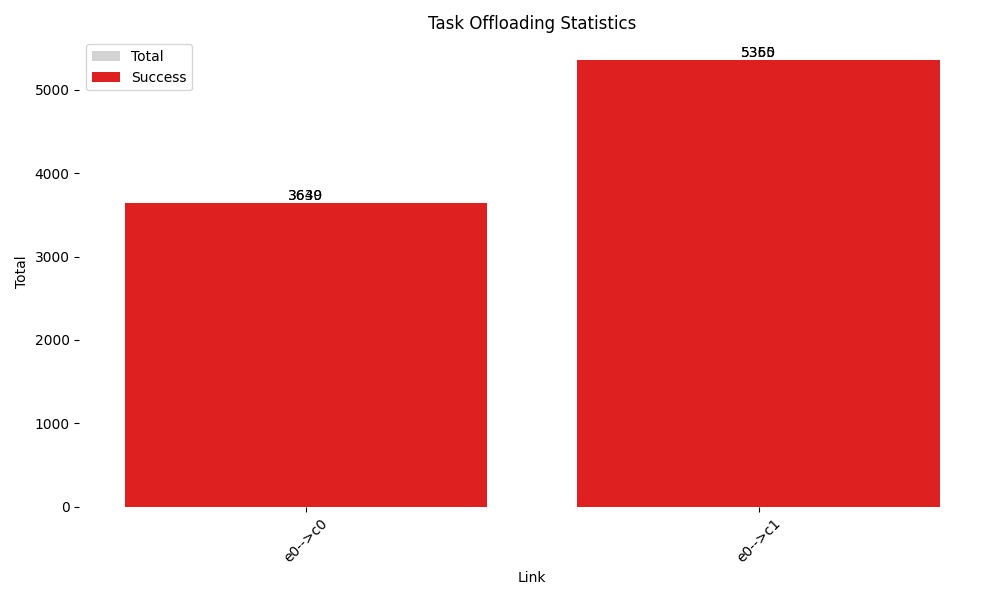
\includegraphics[width=0.5\linewidth]{figs/mlp_task_offloading_statistics.png}
    \caption{Task Offloading Statistics for MLP-based DQRL}
    \label{fig:mlp-task-offloading-stats}
\end{figure}

As depicted in Figure~\ref{fig:mlp-task-offloading-stats}, the MLP policy aggressively exploits cloud nodes to minimize task throw rate (TTR) and latency, aligning with the high \(\lambda_0\) (failure penalty) and \(\lambda_1\) (latency) in the reward. However, by underutilizing fog devices, energy costs shift heavily to cloud nodes.



\subsubsection{Transformer-Based DQRL (TaskFormer)}
While NodeFormer and TaskFormer both show improvements over MLP-based solutions, TaskFormer typically outperforms NodeFormer due to its explicit handling of task attributes.

\begin{figure}[H]
    \centering
    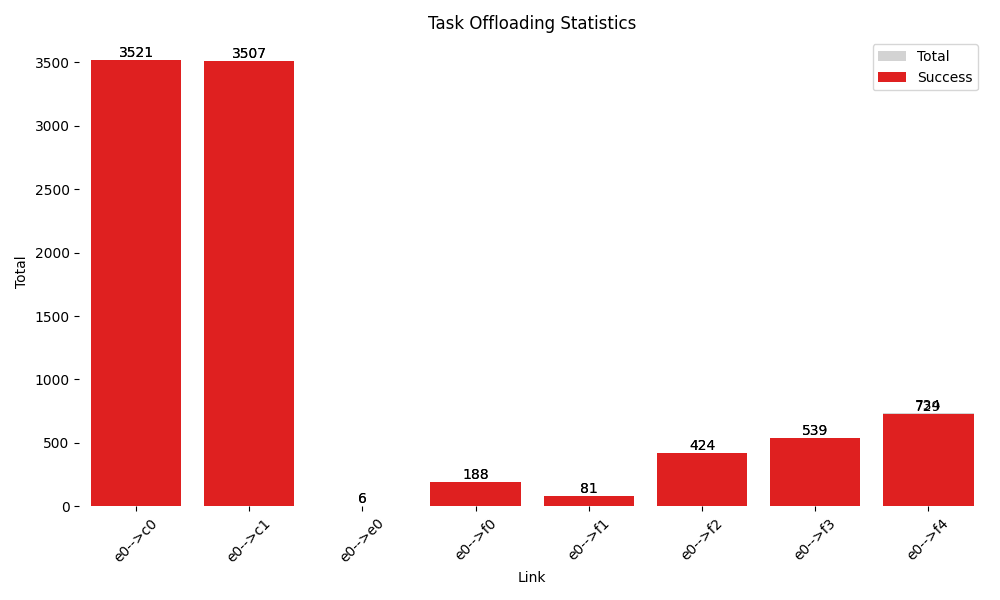
\includegraphics[width=0.5\linewidth]{figs/taskformer_offloading_statistics.png}
    \caption{Task Offloading Statistics for Transformer-based DQRL (TaskFormer)}
    \label{fig:taskformer-offloading-stats}
\end{figure}

\begin{figure}[H]
    \centering
    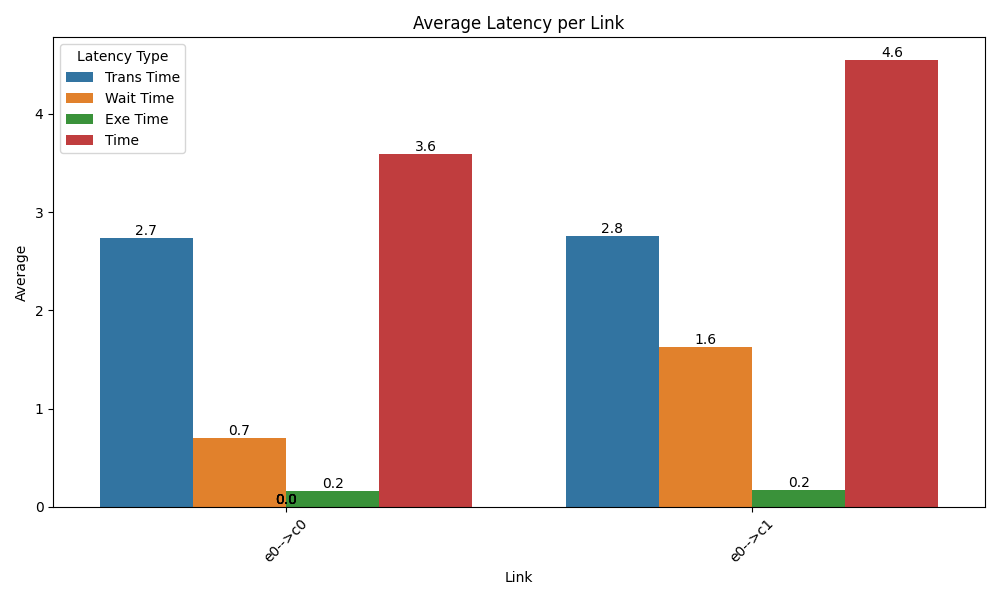
\includegraphics[width=0.5\linewidth]{figs/mlp_avg_latency_per_link.png}
    \caption{Average Latency per Link for MLP-based DQRL}
    \label{fig:mlp-avg-latency}
\end{figure}

\begin{figure}[H]
    \centering
    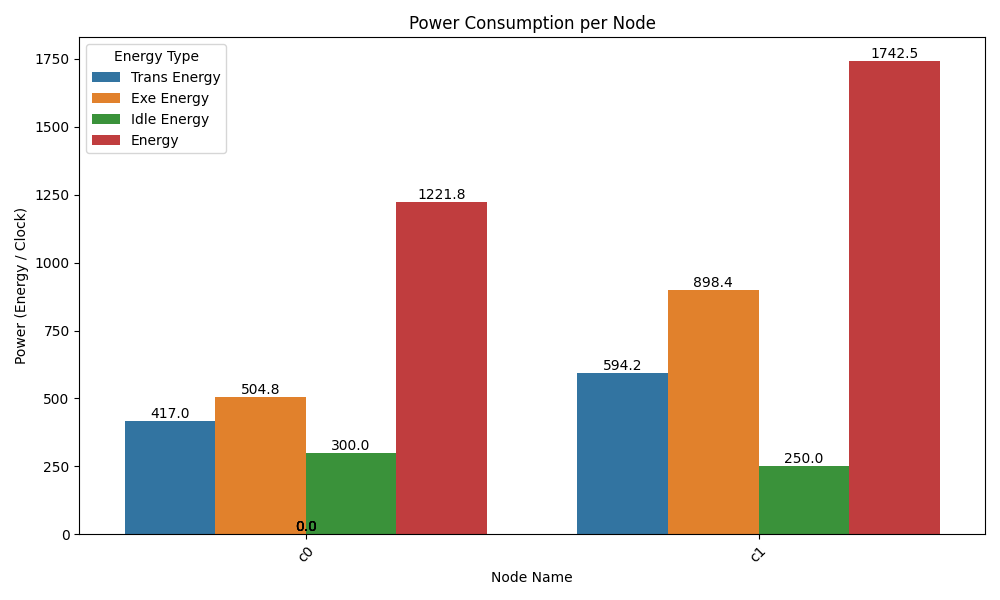
\includegraphics[width=0.5\linewidth]{figs/mlp_power_consumption_per_node.png}
    \caption{Power Consumption per Node for MLP-based DQRL}
    \label{fig:mlp-power-consumption}
\end{figure}

Figures~\ref{fig:mlp-avg-latency} and \ref{fig:mlp-power-consumption} confirm that clouds handle most tasks, yielding minimal latency but higher power usage on those nodes. This trade-off resonates with the single-objective focus of DQRL.
\subsubsection{Transformer-Based DQRL (TaskFormer)}

In Figure~\ref{fig:taskformer-offloading-stats}, TaskFormer still favors cloud nodes but also judiciously employs fog resources when cloud queues rise or tasks demand lower-latency local processing.

\begin{figure}[H]
    \centering
    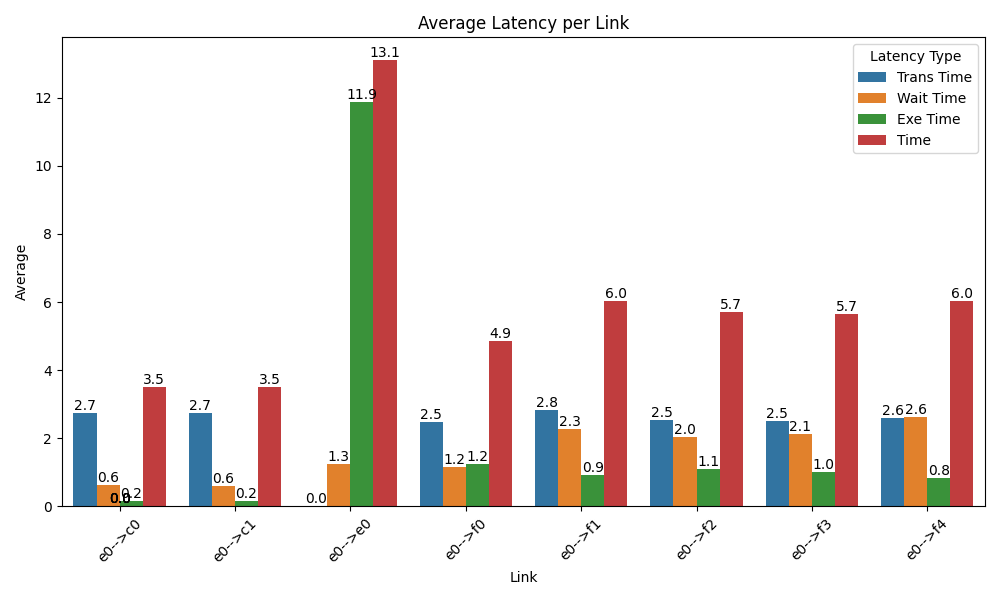
\includegraphics[width=0.5\linewidth]{figs/taskformer_avg_latency_per_link.png}
    \caption{Average Latency per Link for Transformer-based DQRL (TaskFormer)}
    \label{fig:taskformer-avg-latency}
\end{figure}

This balanced allocation is apparent in Figure~\ref{fig:taskformer-avg-latency}, where even edge nodes occasionally participate, though only for specific use cases (e.g., small or time-sensitive tasks). 

\begin{figure}[H]
    \centering
    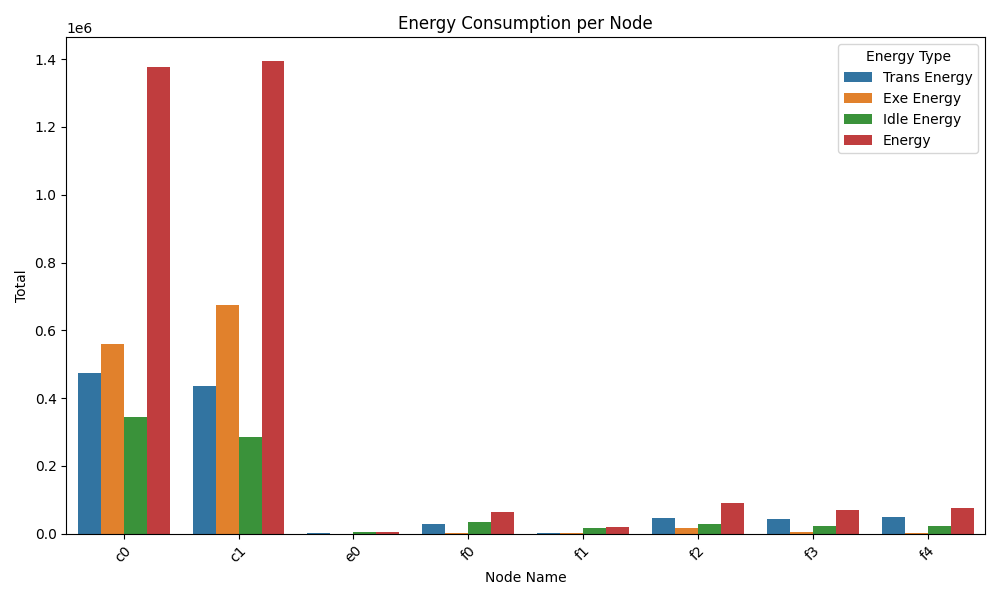
\includegraphics[width=0.5\linewidth]{figs/taskformer_energy_consumption_per_node.png}
    \caption{Energy Consumption per Node for Transformer-based DQRL (TaskFormer)}
    \label{fig:taskformer-energy-consumption}
\end{figure}

Figures~\ref{fig:taskformer-energy-consumption} and \ref{fig:taskformer-cpu-frequency} illustrate that cloud nodes still dominate in both power usage and CPU utilization, aligning with high resource availability and the reward's emphasis on minimizing task failures and latency. Fog nodes remain partially used, mitigating some congestion on the cloud.

\begin{figure}[H]
    \centering
    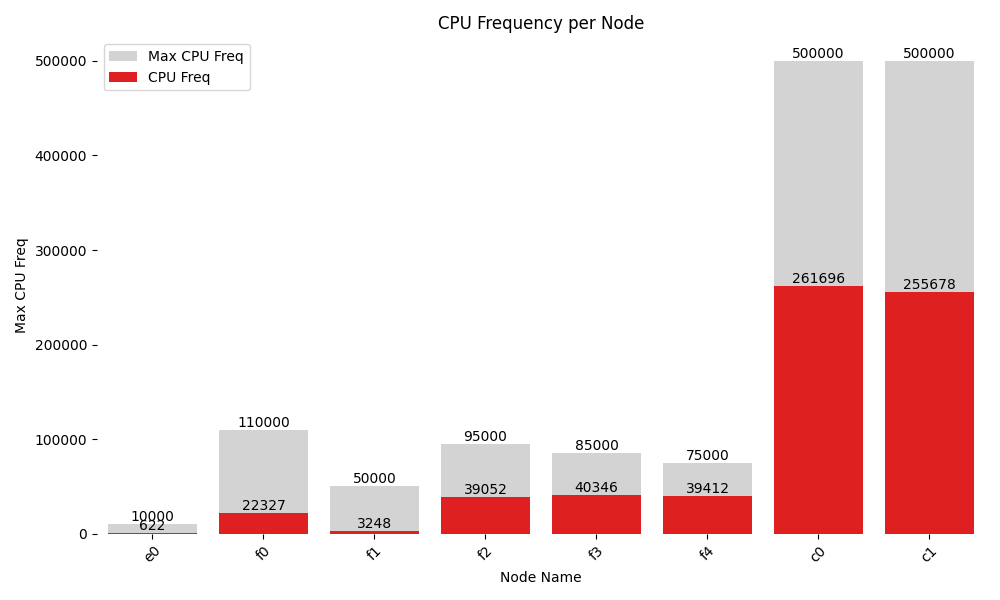
\includegraphics[width=0.5\linewidth]{figs/taskformer_cpu_frequency_per_node.png}
    \caption{CPU Frequency per Node for Transformer-based DQRL (TaskFormer)}
    \label{fig:taskformer-cpu-frequency}
\end{figure}




DECRERIR SE QU'ON VOIT 

\begin{table*}[htbp]
\centering
\caption{Comparison of Offloading Strategies with Task Throw Rate (TTR), Latency (\(L\)), and Energy (\(E\)) on Pakistan test set.
Best results are in \textbf{bold}, second-best are \underline{underlined}.}
\label{tab:results_comparison}
\begin{tabular}{lccc}
\toprule
\textbf{Offloading Strategies} & \textbf{TTR (\%)} & \textbf{Latency (s)} & \textbf{Energy (W)} \\
\midrule

Random 
 & 16.32 
 & 19.9182 
 & 231.9162 \\
 
Round Robin 
 & 14.98 
 & 18.3637 
 & \textbf{239.9348} \\
 
Greedy 
 & 0.19 
 & 4.3936 
 & 338.6719 \\
 
NSGA2 + MLP 
 & \underline{0.07} 
 & 4.1625 
 & 384.9381 \\  % Second-best TTR (tie)
 
NPGA + MLP 
 & 0.14 
 & 4.2422 
 & 380.7835 \\
 
DQRL + MLP 
 & \underline{0.07} 
 & 4.1625 
 & 384.9384 \\  % Second-best TTR (tie)
 
DQRL + NodeFormer 
 & \textbf{0.00} 
 & \underline{3.4534} 
 & 374.6757 \\ % Best TTR (tie), second-best latency
 
DQRL + TaskFormer 
 & \textbf{0.00} 
 & \textbf{3.1041} 
 & 348.8695 \\ % Best TTR (tie), best latency, best energy
 
\bottomrule
\end{tabular}
\end{table*}

CRITIQUE 

OPTIMISATION MUTIti


RR RANDOM PAS COMPARQBLE, MQIS GREEDY OUI

CONFIRMER LE TABLEU

CONFIRMER AUE TASKFORMER 



While many existing offloading solutions rely on synthetic datasets and focus on Multi-access or Vehicular Edge Computing (MEC/VEC) scenarios \cite{fahimullah_review_2022, tu_task_2022, gholipour_tpto_2023}, research specifically targeting fog computing remains limited. In particular, models such as Deep Neural Networks (DNNs) \cite{sarkar_deep_2022} and Deep Q-Learning (DQL) \cite{jiang_reinforcement_2021} have rarely been evaluated in realistic fog environments using real-world data. 

As GA are often static, such as \cite{bernard_d-npga_2024, pakmehr_etfc_2024}, meaning that it's can not be employ in realtime and can only converge throw iteration on the same sumilation , or envireenemt where the task and them order are static , making it really complexe to use it in real world application.

Transformers base DL technique still peu explored, even if it's the state of art in many fields, some exploration are interesting;  however,  and with basic action, such as TPTO \cite{gholipour_tpto_2023} wich are build to with 2 actions, the task is offload to cloud or on edge.